%%%%%%%%%%%%%%%%%%%%%%%%%%%%%%%%%%%%%%%%%
% baposter Landscape Poster
% LaTeX Template
% Version 1.0 (11/06/13)
%
% baposter Class Created by:
% Brian Amberg (baposter@brian-amberg.de)
%
% This template has been downloaded from:
% http://www.LaTeXTemplates.com and modified by Antonius Torode
%
% License:
% CC BY-NC-SA 3.0 (http://creativecommons.org/licenses/by-nc-sa/3.0/)
%
%%%%%%%%%%%%%%%%%%%%%%%%%%%%%%%%%%%%%%%%%

%----------------------------------------------------------------------------------------
%	PACKAGES AND OTHER DOCUMENT CONFIGURATIONS
%----------------------------------------------------------------------------------------

\documentclass[landscape,a0paper,fontscale=0.285]{baposter} % Adjust the font scale/size here

\usepackage{graphicx} % Required for including images
\graphicspath{{figures/}} % Directory in which figures are stored

\usepackage{amsmath} % For typesetting math
\usepackage{amssymb} % Adds new symbols to be used in math mode

\usepackage{booktabs} % Top and bottom rules for tables
\usepackage{enumitem} % Used to reduce itemize/enumerate spacing
\usepackage{palatino} % Use the Palatino font
\usepackage[font=small,labelfont=bf]{caption} % Required for specifying captions to tables and figures

\usepackage{multicol} % Required for multiple columns
\setlength{\columnsep}{1.5em} % Slightly increase the space between columns
\setlength{\columnseprule}{0mm} % No horizontal rule between columns

\usepackage{tikz} % Required for flow chart
\usetikzlibrary{shapes,arrows} % Tikz libraries required for the flow chart in the template

\newcommand{\compresslist}{ % Define a command to reduce spacing within itemize/enumerate environments, this is used right after \begin{itemize} or \begin{enumerate}
\setlength{\itemsep}{1pt}
\setlength{\parskip}{0pt}
\setlength{\parsep}{0pt}
}

\definecolor{lightblue}{rgb}{0.145,0.6666,1} % Defines the color used for content box headers


\begin{document}
	
\background{%
	\begin{tikzpicture}
	[remember picture,overlay]\node[opacity=1] at (current page.center) {
\includegraphics[width=\paperwidth,height=\paperheight]{BG3.jpg}};
	\end{tikzpicture}%
}

\begin{poster}
{
headerborder=closed, % Adds a border around the header of content boxes
colspacing=1em, % Column spacing
background=user,
%bgColorOne=white, % Background color for the gradient on the left side of the poster
%bgColorTwo=white, % Background color for the gradient on the right side of the poster
borderColor=lightblue, % Border color
headerColorOne=black, % Background color for the header in the content boxes (left side)
headerColorTwo=lightblue, % Background color for the header in the content boxes (right side)
headerFontColor=white, % Text color for the header text in the content boxes
boxColorOne=white, % Background color of the content boxes
textborder=roundedleft, % Format of the border around content boxes, can be: none, bars, coils, triangles, rectangle, rounded, roundedsmall, roundedright or faded
eyecatcher=true, % Set to false for ignoring the left logo in the title and move the title left
headerheight=0.1\textheight, % Height of the header
headershape=roundedright, % Specify the rounded corner in the content box headers, can be: rectangle, small-rounded, roundedright, roundedleft or rounded
headerfont=\Large\bf\textsc, % Large, bold and sans serif font in the headers of content boxes
%textfont={\setlength{\parindent}{1.5em}}, % Uncomment for paragraph indentation
linewidth=2pt % Width of the border lines around content boxes
}
%----------------------------------------------------------------------------------------
%	TITLE SECTION 
%----------------------------------------------------------------------------------------
%
{
\includegraphics[height=4em]{MSU.jpg}} % First university/lab logo on the left
{\bf\textsc{Zeeman Effect}\vspace{0.5em}} % Poster title
{\textsc{Antonius Torode and Eric Aboud -  \hspace{12pt} Michigan State University \\ Department of Physics \& Astronomy}} % Author names and institution
{
\includegraphics[height=4em]{MSU.jpg}} % Second university/lab logo on the right

%----------------------------------------------------------------------------------------
%	OBJECTIVES
%----------------------------------------------------------------------------------------

\headerbox{Introduction \& History}{name=objectives,column=0,row=0}{



\vspace{0.3em} % When there are two boxes, some whitespace may need to be added if the one on the right has more content
}

%----------------------------------------------------------------------------------------
%	Discovery & Properties
%----------------------------------------------------------------------------------------

\headerbox{Discovery \& Properties }{name=introduction,column=3,row=0,bottomaligned=objectives}{


}

%----------------------------------------------------------------------------------------
%	Derivation of the Casimir Force
%----------------------------------------------------------------------------------------

\headerbox{Derivation of Induced Electric Field}{name=results,column=1,span=2,row=0}{

\begin{multicols}{2}

\end{multicols}
}

%----------------------------------------------------------------------------------------
%	REFERENCES
%----------------------------------------------------------------------------------------

\headerbox{References}{name=references,column=0,above=bottom}{


\scriptsize{ % Reduce the font size in this block
\begin{enumerate}
\itemsep0em 
\item John Baez on the number 24. The Rankin Lectures 2008. Youtube. John Baez. University of California. 16 May. 2012. Web. \label{baez}
\item Gibbs, Philip. "What Is the Casimir Effect?" The Casimir Effect. University of California, 1997. Web. 16 Oct. 2016. 
\item Ramanujan Aiyangar, Srinivasa, 1887-l  920. Ramanujans notebooks. Mathematics-Collected works. 1. Berndt, Bruce C., 1939- II. Title. QA3. R33. 1985. 510. 84-20201 \label{ramanujin}

\end{enumerate}
}}

%----------------------------------------------------------------------------------------
%	Addendum and Final Remarks
%----------------------------------------------------------------------------------------

\headerbox{Addendum and Final Remarks }{name=futureresearch,column=1,span=2,aligned=references,above=bottom}{ % This block is as tall as the references block
\begin{multicols}{2}

\end{multicols}
}

%----------------------------------------------------------------------------------------
%	References RIGHT
%----------------------------------------------------------------------------------------

\headerbox{References}{name=contact,column=3,aligned=references,above=bottom}{ % This block is as tall as the references block

\scriptsize{ % Reduce the font size in this block
	\begin{enumerate}
		\setcounter{enumi}{3}
		\itemsep0em 
		\item Casimir Effect \& Black Holes - Sixty Symbols. Prod. Brady Haran. Perf. Mike Merrifield Ph.D. Youtube. University of Nottingham, 20 Mar. 2014. Web. 
		\item H.B.G. Casimir, Proc. Kon. Ned. Akad. Wetensch. B51, 793 (1948) \label{casimir}
		\item Sum of Natural Numbers (second proof and extra footage). Prod. Brady Haran. Perf. Ed Copeland Ph.D and Tony Padilla Ph.D. Youtube. University of Nottingham, 11 Jan. 2015. Wb.
	\end{enumerate}
}}

%----------------------------------------------------------------------------------------
%	Implications and Applications
%----------------------------------------------------------------------------------------

\headerbox{Implications and Applications}{name=conclusion,column=1,span=2,row=0,below=results,above=references}{

\begin{multicols}{2}

\end{multicols}
}

%----------------------------------------------------------------------------------------
%	Astounding Mathematics
%----------------------------------------------------------------------------------------

\headerbox{Computational Models}{name=method,column=3,below=objectives,bottomaligned=conclusion}{ % This block's bottom aligns with the bottom of the conclusion block
\small{
	
\begin{center}
	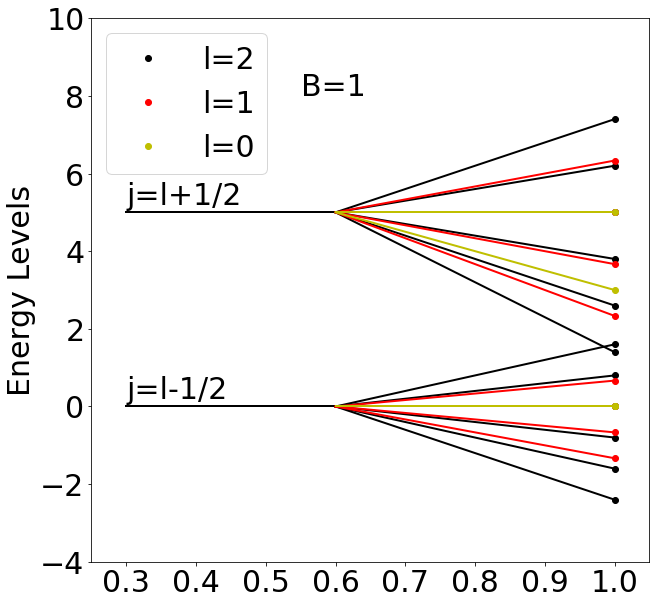
\includegraphics[width=0.7\linewidth]{figures/Bis1}
	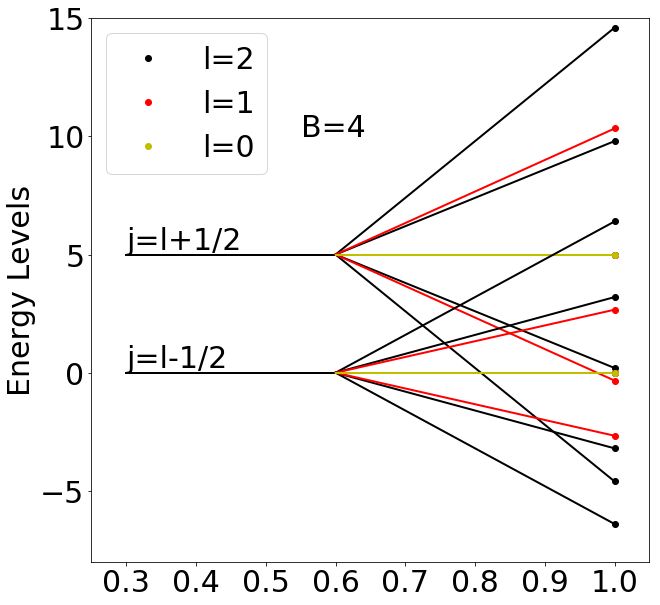
\includegraphics[width=0.7\linewidth]{figures/Bis4}
\end{center}
	
	

}}

%----------------------------------------------------------------------------------------
%	Analytic Continuation
%----------------------------------------------------------------------------------------

\headerbox{Land\'{e}  g Factor}{name=results2,column=0,below=objectives,bottomaligned=conclusion}{ % This block's bottom aligns with the bottom of the conclusion block
\small{

}}

%----------------------------------------------------------------------------------------

\end{poster}

\end{document}